
\documentclass[a4paper,12pt]{article}
\usepackage[utf8]{inputenc}
\usepackage[T1]{fontenc}
\usepackage{graphicx}
\usepackage{hyperref}
\title{Esercitazioni 1--6 - Analisi di Rete}
\author{}
\date{}

\begin{document}
\maketitle

%% Esercizio 1
\section*{Esercizio 1}
\begin{enumerate}
  \item \textbf{Che tipo di protocollo di livello Data-link è utilizzato? Come fa Wireshark a capirlo?}\\
    Utilizza il protocollo Ethernet. Wireshark lo capisce perché nel pacchetto è presente il campo \emph{EtherType}.
  \item \textbf{Disegnare la PDU di livello Data-link indicando il valore dei vari campi.}\\
    \begin{figure}[h]
      \centering
      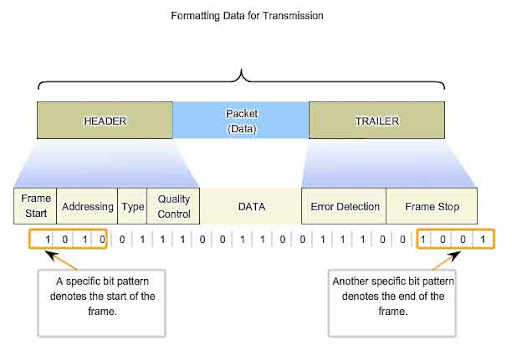
\includegraphics[width=0.8\linewidth]{src/foto_PDU_DataLink.png}
      \caption{PDU Data-link}
    \end{figure}
  \item \textbf{Qual è il MAC sorgente? Di che tipo è: unicast o broadcast?}\\
    Il MAC sorgente è \texttt{00:e0:81:24:dd:64} ed è di tipo \emph{unicast}.
  \item \textbf{Qual è il MAC destinazione? Di che tipo è: unicast o broadcast?}\\
    Il MAC destinazione è \texttt{ff:ff:ff:ff:ff:ff} ed è di tipo \emph{broadcast}.
  \item \textbf{Che tipo di protocollo di livello Network è utilizzato? Come fa Wireshark a capirlo?}\\
    Viene utilizzato il protocollo IPv4. Wireshark lo capisce leggendo il campo \emph{Type} nell'header Data-link.
  \item \textbf{Qual è la lunghezza dell'header IP?}\\
    La lunghezza dell'header IP è di 20 byte.
  \item \textbf{Quali sono gli indirizzi IP sorgente e destinazione?}\\
    IP sorgente: \texttt{157.27.252.223}\\
    IP destinazione: \texttt{157.27.252.255}
  \item \textbf{Che tipo di protocollo di livello trasporto è contenuto in IP? Come fa Wireshark a capirlo?}\\
    Viene usato il protocollo UDP. Wireshark lo capisce leggendo il campo \emph{Protocol} nell'header IP.
  \item \textbf{Quali sono le porte sorgente e destinazione a livello trasporto?}\\
    Porta sorgente: \texttt{631}\\
    Porta destinazione: \texttt{631}
  \item \textbf{Creare un filtro per visualizzare solo i pacchetti che hanno ARP come protocollo.}\\
    \texttt{arp}
    \begin{figure}[h]
      \centering
      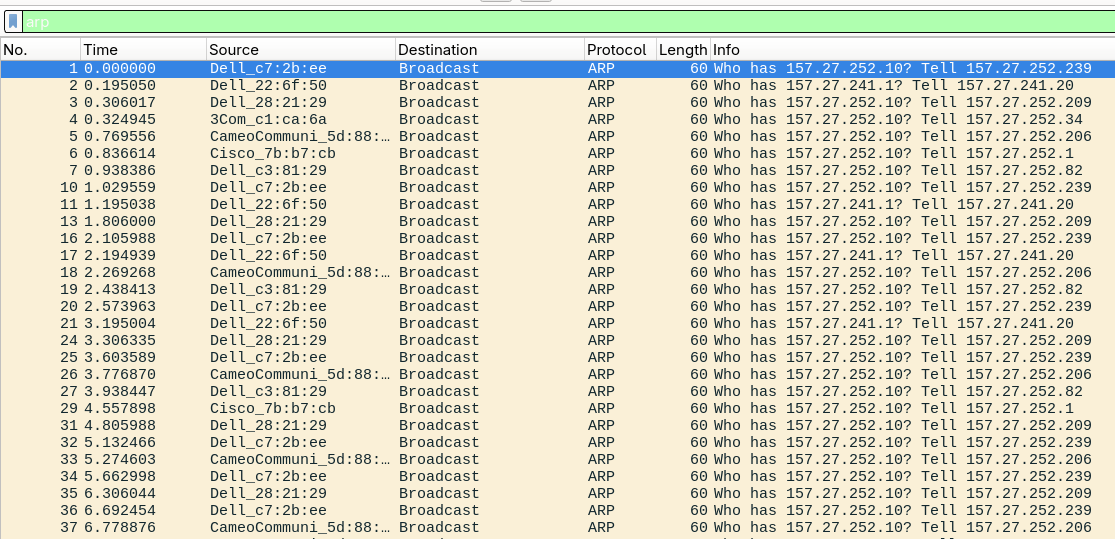
\includegraphics[width=0.6\linewidth]{src/filtroARP.png}
      \caption{Filtro ARP}
    \end{figure}
  \item \textbf{Dopo aver applicato il filtro precedente qual è la percentuale di pacchetti che rimangono visualizzati rispetto al totale?}\\
    63\% (173 pacchetti su 272)
  \item \textbf{Creare un filtro per visualizzare solo i pacchetti che hanno destinazione MAC \texttt{00:01:e6:57:4b:e0}.}\\
    \texttt{eth.dst == 00:01:e6:57:4b:e0}
    \begin{figure}[h]
      \centering
      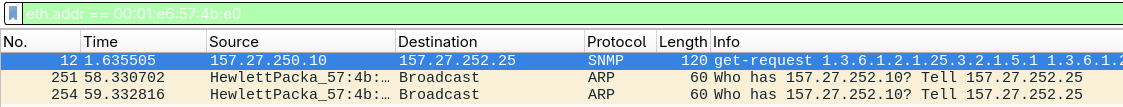
\includegraphics[width=0.6\linewidth]{src/filtro_dest_MAC.png}
      \caption{Filtro destinazione MAC specifico}
    \end{figure}
  \item \textbf{Dopo aver applicato il filtro precedente qual è la percentuale di pacchetti che rimangono visualizzati rispetto al totale?}\\
    0.4\% (1 pacchetto su 272)
  \item \textbf{Creare un filtro per visualizzare solo i pacchetti che hanno destinazione MAC broadcast.}\\
    \texttt{eth.dst == ff:ff:ff:ff:ff:ff}
    \begin{figure}[h]
      \centering
      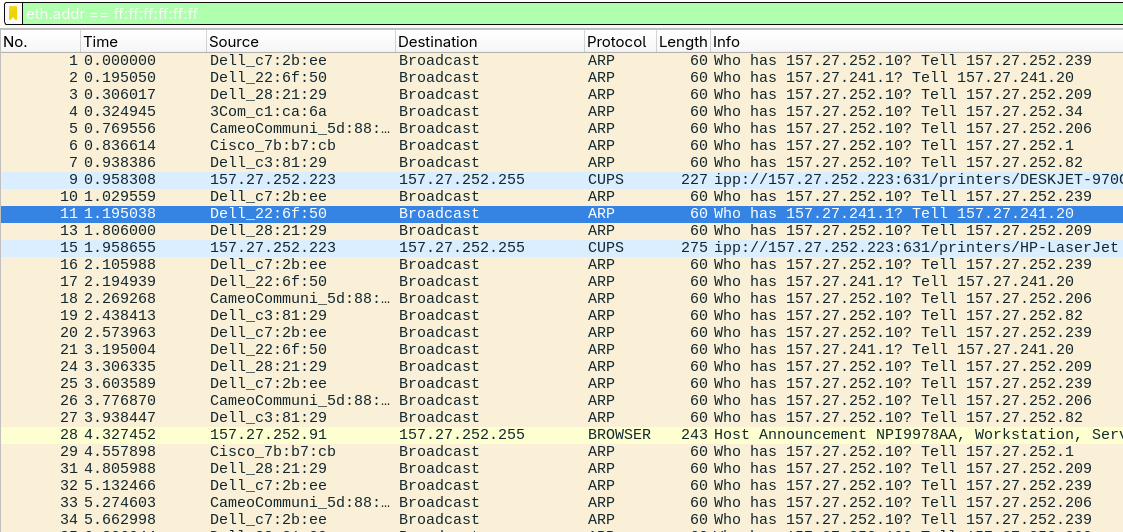
\includegraphics[width=0.6\linewidth]{src/filtroMAC_broadcast.png}
      \caption{Filtro MAC broadcast}
    \end{figure}
  \item \textbf{Dopo aver applicato il filtro precedente qual è la percentuale di pacchetti che rimangono visualizzati rispetto al totale? Sono molti? Perché?}\\
    83.8\% (228 pacchetti su 272). Sono molti perché ci sono state molte assegnazioni IP tramite protocollo ARP.
\end{enumerate}

%% Esercizio 2
\section*{Esercizio 2}
\begin{enumerate}
  \item \textbf{Colorare di rosso tutti i pacchetti che contengono UDP e di verde tutti i pacchetti che contengono TCP.}\\
    \begin{figure}[h]
      \centering
      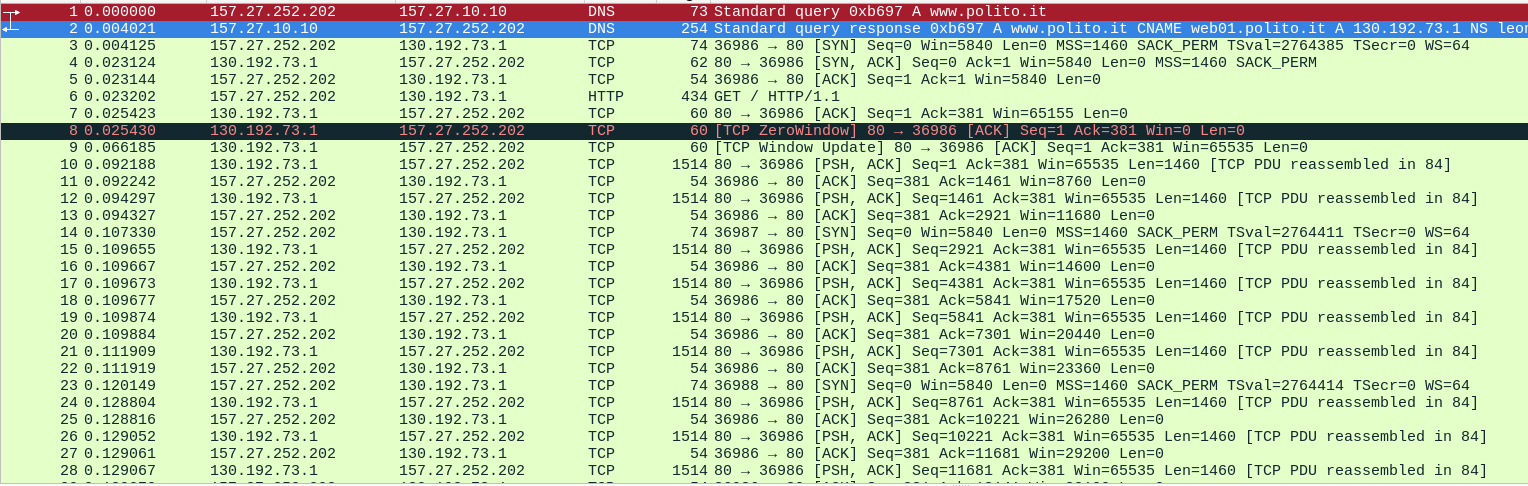
\includegraphics[width=0.8\linewidth]{src/filtro_rosso.png}
      \caption{Regole di colorazione UDP/TCP}
    \end{figure}
  \item \textbf{Cosa contengono i primi due pacchetti della sessione di cattura?}\\
    \textbf{Pacchetto 1:}
    \begin{itemize}
      \item IP sorgente: \texttt{157.27.252.202}
      \item IP destinazione: \texttt{157.27.10.10}
      \item Trasporto: UDP
      \item Applicazione: DNS (www.polito.it)
    \end{itemize}
    \textbf{Pacchetto 2:}
    \begin{itemize}
      \item IP sorgente: \texttt{157.27.10.10}
      \item IP destinazione: \texttt{157.27.252.202}
      \item Trasporto: UDP
      \item Applicazione: DNS (web01.polito.it $\to$ 130.192.73.1)
    \end{itemize}
  \item \textbf{Prendere in considerazione il pacchetto n. 3.}\\
    \begin{itemize}
      \item IP sorgente: \texttt{157.27.252.202}
      \item IP destinazione: \texttt{130.192.73.1}
      \item Trasporto: TCP
      \item Applicazione: risposta alla ricerca DNS
    \end{itemize}
  \item \textbf{Prendere in considerazione il pacchetto n. 6.}\\
    \begin{itemize}
      \item IP sorgente: \texttt{157.27.252.202}
      \item IP destinazione: \texttt{130.192.73.1}
      \item Trasporto: TCP
      \item Applicazione: HTTP
      \item I tre pacchetti precedenti sono il Three Way Handshake (flag SEQ e ACK).
    \end{itemize}
  \item \textbf{Filtro per pacchetti TCP (inclusi HTTP), numero pacchetti:}\\
    807 su 823
  \item \textbf{Filtro per pacchetti TCP (esclusi HTTP), numero pacchetti e percentuale:}\\
    673 su 823 (81,8\%). Sono i pacchetti TCP di handshake; se DNS usasse TCP, sarebbero stati generati 6 pacchetti in più, rallentando.
  \item \textbf{Seguire lo stream TCP: cosa si può leggere?}\\
    Si possono leggere le varie richieste HTTP GET.
\end{enumerate}

%% Esercizio 3
\section*{Esercizio 3}
\begin{enumerate}
  \item \textbf{Protocolli di livello Applicazione per trasporto:}\\
    UDP: DNS \\
    TCP: HTTP, FTP, SSH
  \item \textbf{Analisi di diversi stream TCP:}\\
    \begin{figure}[h]
      \centering
      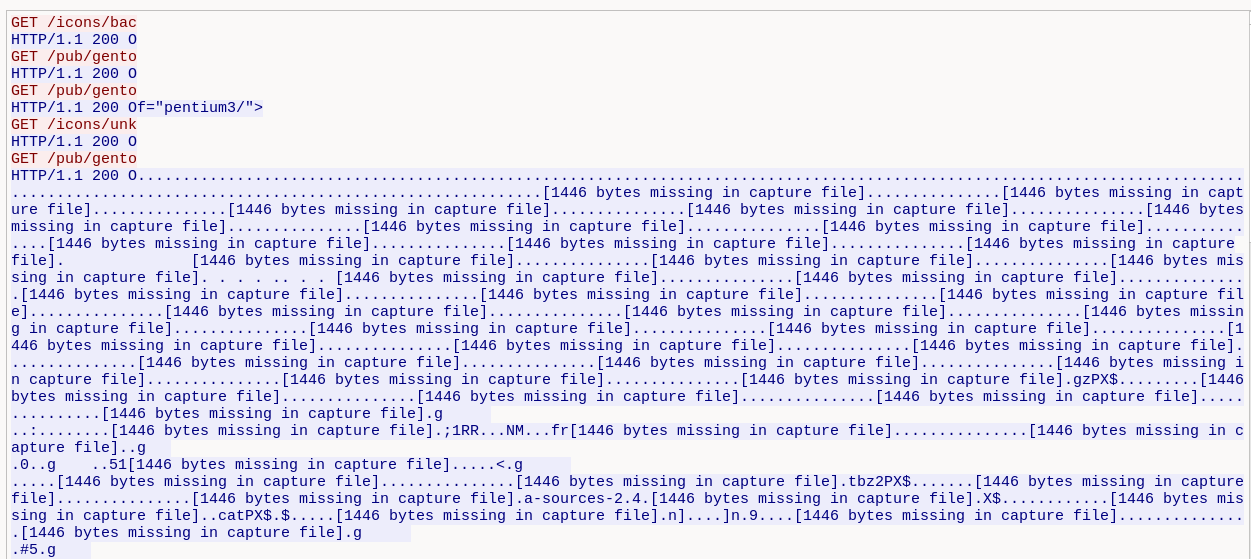
\includegraphics[width=0.8\linewidth]{src/streamTCP.png}
      \caption{Esempio di stream TCP}
    \end{figure}
  \item \textbf{Differenza FTP vs SSH:}\\
    Sì, la differenza è che SSH è criptato.
\end{enumerate}

%% Esercizio 4
\section*{Esercizio 4}
\begin{enumerate}
  \item \textbf{Numero richieste ping e risposte:}\\
    22 su 3215
  \item \textbf{IP sorgente e destinazione delle richieste ICMP e intestatari:}\\
    IP sorgente: \texttt{157.27.143.46} \\
    IP destinazione: \texttt{216.58.211.196} (www.google.com)
  \item \textbf{RTT medio e variazione (google vs gateway):}\\
    RTT gateway: 0.028\,ms \\
    RTT Google: 5.75\,ms \\
    Il gateway mostra RTT minore essendo interno alla rete locale.
\end{enumerate}

%% Esercizio 5
\section*{Esercizio 5}
\begin{enumerate}
  \item \textbf{Interfacce dei router attraversati:}\\
    \begin{figure}[h]
      \centering
      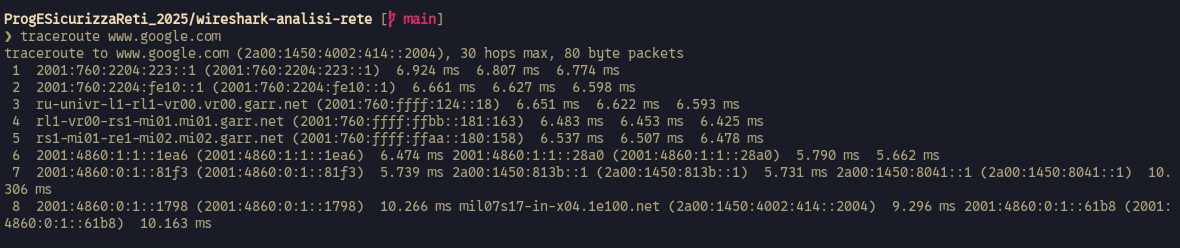
\includegraphics[width=0.8\linewidth]{src/traceroute.png}
      \caption{Output del traceroute}
    \end{figure}
  \item \textbf{Organizzazioni intestatarie degli IP:}\\
    Vedi annotazioni nel tracciato (fig.\,traceroute).
\end{enumerate}

%% Esercizio 6
\section*{Esercizio 6}
\begin{enumerate}
  \item \textbf{Interfacce attive, IP e netmask:}\\
    \begin{figure}[h]
      \centering
      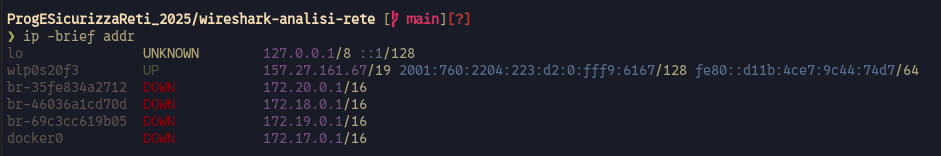
\includegraphics[width=0.6\linewidth]{src/interfaccie.png}
      \caption{Interfacce attive sul PC}
    \end{figure}
  \item \textbf{IP di www.univr.it:}\\
    Ricavato tramite nslookup o comando equivalente (vedi fig.\,interfaccie).
\end{enumerate}

\end{document}
